
\documentclass[tikz,border=5pt]{standalone}
\usepackage{tikz}
\usetikzlibrary{positioning}

\begin{document}

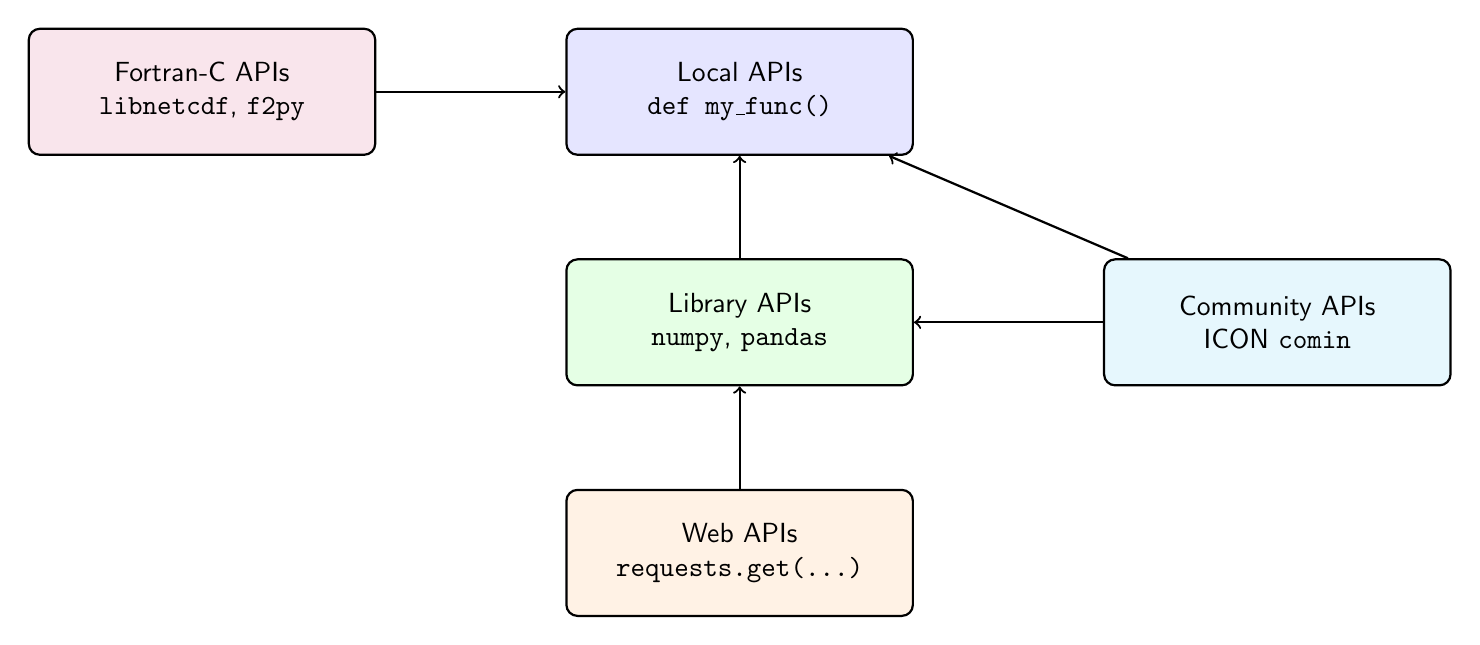
\begin{tikzpicture}[
  node distance=1.3cm and 2.4cm,
  every node/.style={font=\sffamily},
  box/.style={draw, thick, rounded corners, align=center, minimum width=4.4cm, minimum height=1.6cm},
  arrow/.style={->, thick}
]

% Top
\node[box, fill=blue!10] (local) {Local APIs\\\texttt{def my\_func()}};

% Middle row
\node[box, fill=green!10, below=of local] (library) {Library APIs\\\texttt{numpy}, \texttt{pandas}};
\node[box, fill=orange!10, below=of library] (web) {Web APIs\\\texttt{requests.get(...)}};

% Bottom row
\node[box, fill=purple!10, left=of local] (fortran) {Fortran-C APIs\\\texttt{libnetcdf}, \texttt{f2py}};
\node[box, fill=cyan!10, right=of library] (comin) {Community APIs\\ICON \texttt{comin}};

% Arrows
\draw[arrow] (library) -- (local);
\draw[arrow] (web) -- (library);
\draw[arrow] (fortran) -- (local);
\draw[arrow] (comin) -- (library);
\draw[arrow] (comin) -- (local);

\end{tikzpicture}

\end{document}

